\documentclass[conference]{IEEEtran}
\IEEEoverridecommandlockouts
% The preceding line is only needed to identify funding in the first footnote. If that is unneeded, please comment it out.
\usepackage{cite}
\usepackage{amsmath,amssymb,amsfonts}
\usepackage{algorithmic}
\usepackage{graphicx}
\usepackage{textcomp}
\usepackage{xcolor}
\usepackage{pythonhighlight}
\def\BibTeX{{\rm B\kern-.05em{\sc i\kern-.025em b}\kern-.08em
    T\kern-.1667em\lower.7ex\hbox{E}\kern-.125emX}}
\begin{document}

\title{Single Image Super Resolution: Exploring }

\author{\IEEEauthorblockN{Jerry Duncan}
  \IEEEauthorblockA{\textit{Electrical Engineering and Computer Science Department} \\
    \textit{University of Tennessee}\\
    Knoxville, USA \\
    jdunca51@vols.utk.edu}
}

\maketitle

\begin{abstract}
  Data is being created at an endless rate, faster than we can store all of it.
  Consequently, images are often greatly compressed and lose a large portion of their quality and crispness.
  Single Image Super Resolution aims to change that by using Deep Convolutional Neural Networks to upscale low resolution images.
  In this work we're expanding upon that to bring Single Image Super Resolution to low compute devices while still keeping better upscaling performance than simple bicubic upscaling.
  We managed to get a Peak Signal-to-Noise Ratio of 29.85 dB using a network with less than 1,000 parameters compared to bicubic's 29.24 dB.
\end{abstract}

\begin{IEEEkeywords}
  super resolution
\end{IEEEkeywords}

\section{Introduction}

In the Information Age, data is being created at an endless rate and will soon be created faster than we can store all of it.
To help compensate for this problem, images are often stored in less than ideal formats, like JPEG where they're compressed to save space.
When converting a high-quality, high-resolution image to JPEG, it inherently loses image quality in exchange for faster transfer speeds and less disk space.
JPEG, other image compression techniques, and downscaling filters all cause images to lose large amounts of crispness and information that is unrecoverable.
Because of that, ways to upscale compressed images to their original quality has been a hot topic of research since the beginning of the Internet.

For years, we've been looking for more classical solutions to upscaling images while keeping crisp image clarity and interpolating features that make sense.
Unfortunately, most classical solutions fail in a variety of ways.
Upscaling filters such as bicubic and bilinear leave images blurry and lacking in definition after upscaling.
And the Lanczos filter, one thought to be the best all-purpose filter, leaves a lot to be desired \cite{b4}.

Recently, Deep Convolutional Neural Networks have been architected to learn how to upscale images more accurately than all other image resampling methods \cite{b5}, deemed "Super Resolution".
They train on specifically selected high resolution images and their low resolution counterparts.
In doing so, they're able to better recreate high resolution images from low resolution ones, but are typically somewhat costly to train, both in terms of the cost of the hardware to run them and the time in which they take to train.
In today's world, such a setup is too expensive for the overwhelming majority of people.
However, most people own a smartphone that could potentially be leveraged to train one of these networks on-device and then use it on incoming images to help save global bandwidth and network congestion.

In this project, we'll be exploring ways that we can lower the computational cost of the most popular Single Image Super Resolution network described in \cite{b6}.
We'll be taking a look at how few parameters we can get away with while still producing high quality images.
We'll also be taking a look at how well we can boost the network's performance on very small images.

\section{Previous Work}

The field of super resolution has boomed over recent years, with a major increase in publications in 2017.
The first papers focused on using an already existing method to upscale low resolution images like a bicubic filter and then using a CNN to better refine the image \cite{b5}.
While they worked and were already better than standard bicubic upscaling, they were deep networks that were expensive to train with millions of parameters and were generally considered too computationally expensive.
Then, in 2016, W. Shi \textit{et al.} \cite{b6} created the sub-pixel convolution layer which learns an array of upscaling filters to convert low resolution feature maps to high resolution ones.
This discovery created an influx of super resolution papers in the field in the following years.
For this project, we'll be starting with one of those papers that was also pivotal in its ideals.
Deemed the Enhanced Deep Super-Resolution Network (EDSR), it was the first to combine thin residual layers with sub-pixel upscaling and manage to reach a Peak Signal-to-Noise Ratio (PSNR) of 35 db \cite{b1}.


\section{Technical Approach}
The goal of our project is to fine tune an EDSR network to be as thin as possible while achieving a PSNR of 30+ on the CINIC-10 dataset.
The reason for this is that we intend to deploy this network to low compute devices, like phones, if possible so a thin, low parameter network that can perform well on very small images is ideal.
We preprocess our CINIC-10 images by using Matlab's bicubic imresize to create low resolution versions of each image for use in training.

We're using the EDSR architecture as our model, which is better described in Figure \ref{fig:edsr}.
It consists of a global residual connection that's intended to learn what input features are important to keep before upscaling, a variable number of residual blocks, and a sub-pixel convolution layer that learns how to take small feature maps and upscale them to large ones.
Each residual block is slightly different than typical residual blocks or the ones used in previous super resolution networks in that they do not have batch normalization layers and they are not gated by a ReLU after the local residual connection.

We perform training steps by taking a random crop of the low resolution image and passing it through our model.
Then we will use mean absolute error ($\ell_1$ distance) between the upscaled image and the corresponding high resolution patch as the loss we'll use for backpropagation.
After every 1,000 steps we upscale every validation image and calculate the PSNR between them and their high resolution counterparts.
If that PSNR is the best that we have seen then we will create a checkpoint at that step so that we can reload the best model later on.

For our experiments, we will be tweaking a few different parameters.
The first is the sizes of our datasets.
We want to ensure that the network performs well on both datasets before we commit to this architecture and we also want to see how well it can already handle images of varying sizes.
The second is the number of residual blocks we place in between our global residual connection.
We hope that we can achieve a high performance with a low number of residual blocks and consequently a small number of parameters so that we can potentially train our network on a low compute device.
The third and last is the number of filters in each convolutional layer.
We want to try a varying number of filters in both directions, decreasing them to achieve our low compute goal, and increasing them to see if we can increase our PSNR on very small images.

\begin{figure}[htbp]
  \centerline{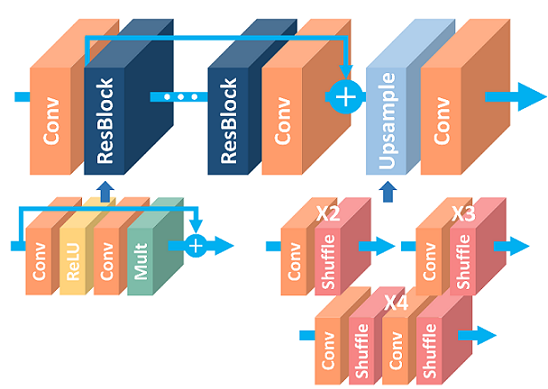
\includegraphics{edsr.PNG}}
  \caption{This is the architecture of an EDSR network. It consists of a global residual connection, a variable number of modified residual blocks (explained in Figure \ref{fig:residual}), and followed by a sub-pixel convolutional layer \cite{b6}. Figure taken from \cite{b5}.}
  \label{fig:edsr}
\end{figure}

\begin{figure}[htbp]
  \centerline{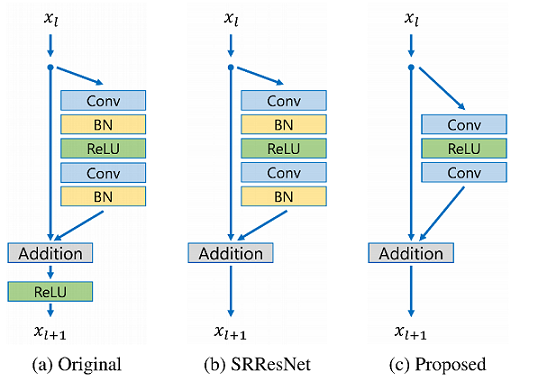
\includegraphics{residual.PNG}}
  \caption{This shows a comparison of typical residual layers and the one used in EDSR. We remove the batch normalization layers as well as the ReLU after the residual connection. Figure taken from \cite{b5}.}
  \label{fig:residual}
\end{figure}

\section{Dataset and Implementation}
We look at two datasets to train single-image super resolution networks on.
The first is DIV2K \cite{b2}, a commonly used super resolution dataset that consists of 800 training and 100 validation high resolution images that have an average width of 1,972 and height of 1,435.
Also provided are the same images downscaled using different downsampling methods and to different scales.
For this project, we'll be looking at the images downscaled using bicubic downsampling and for the most part we'll only be briefly looking at the more extremely scaled images.
The second dataset is CINIC-10 \cite{b3}, a dataset meant to be an intermediate between CIFAR-10 and ImageNet.
It contains hundreds of thousands of images sampled from ImageNet that belong to CIFAR-10 classes and have an average width and height of 256.
For the purposes of our experiments, we use a random number generator to craft a much smaller dataset in the same vein as DIV2K.
Our smaller CINIC-10 dataset contains 800 random training and 100 random validation images chosen randomly and equally from each class (i.e. 80 birds, 80 dogs, etc.).

Most of our experiments are related to reducing the training cost and maximizing the PSNR values of super resolution images.
We'll be mainly tweaking the depth of the network (the number of residual blocks) and the number of convolution filters.

Training time for our networks varies wildly depending on the number of parameters we need to train, but to standardize training across runs, we'll be training each network for 300,000 steps.
Each step of training involves taking a single 96$\times$96 crop from a random high resolution image and the 48$\times$48 corresponding crop from the low resolution image and running forward and backward pass through the network.

Each of our models was trained on its own Tesla V100-SXM2.

\section{Experiments and Results Analysis}
The first experiment we want to run is to see if our network will even work on either of our datasets.
We will use the suggested network hyperparameters from the EDSR paper for these runs, such that there are 16 residual blocks, and every convolutional layer has 64 filters.
We will try this training this network on different sized high and low resolution images from each dataset to see how well it performs as the size of the images decreases.
In Figure \ref{fig:baseline-psnr} and Figure \ref{fig:baseline-loss} we explore the validation PSNR and training loss of the standard network on different sizes of DIV2K and CINIC-10.
We can see a clear trend in both graphs, showing that PSNR deteriorates relative to size and in a similar manner, loss increases.
Fortunately, we're still able to get a PSNR greater than 30 dB on all of the dataset samples tested, so we know that the network will work on extremely small images.
Using normal bicubic upscaling on a downscaled CINIC-10 only gets us a PSNR of 29.24 dB, so that'll be the baseline to compare all of our other networks to.
We can see some examples of images upscaled this way compared to using the model and the original high resolution image in Figure \ref{fig:ex}.
And in Table \ref{tab:baseline}, we can see the highest PSNR value each achieved on the validation set, as well as the lowest loss.
\begin{figure}[htbp]
  \centerline{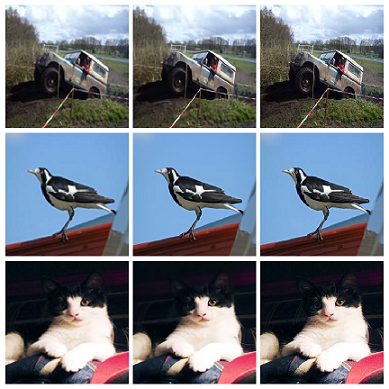
\includegraphics{examples.png}}
  \caption{Left are upscaled to 256x256 from 128x128 using bicubic upscaling, middle are upscaled to 256x256 using the baseline EDSR network, and right are the original high resolution images}
  \label{fig:ex}
\end{figure}

\begin{figure}[htbp]
  \centerline{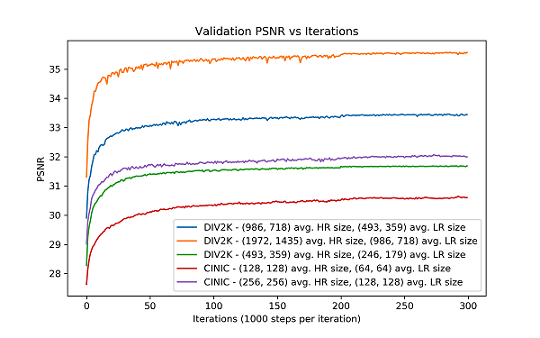
\includegraphics{baseline-psnr.png}}
  \caption{PSNR values on the validation set over time. Each network is using the suggested settings of 16 residual blocks and 64 filters per convolutional layer}
  \label{fig:baseline-psnr}
\end{figure}

\begin{figure}[htbp]
  \centerline{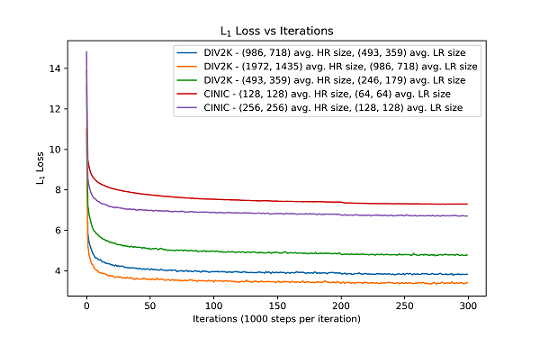
\includegraphics{baseline-loss.png}}
  \caption{Loss values on the training set over time. Each network is using the suggested settings of 16 residual blocks and 64 filters per convolutional layer}
  \label{fig:baseline-loss}
\end{figure}

\begin{table}[htbp]
  \centering
  \caption{Each network tested in this table is the recommended EDSR network.}
  \label{tab:baseline}
  \begin{tabular}{c|c|c|c|c|c}
    Dataset & HR Size    & LR Size  & sec / epoch & PSNR     & $L_1$ Loss \\ \hline
    DIV2K   & 1972, 1435 & 986, 718 & 76.78       & 35.58 dB & 3.34       \\
    DIV2K   & 986, 718   & 493, 359 & 32.29       & 33.46 dB & 3.78       \\
    DIV2K   & 493, 359   & 246, 179 & 32.03       & 31.69 dB & 4.74       \\
    CINIC   & 256, 256   & 128, 128 & 31.93       & 32.07 dB & 6.70       \\
    CINIC   & 128, 128   & 64, 64   & 32.13       & 30.64 dB & 7.28       \\
  \end{tabular}
\end{table}

The next experiment we want to run is to see how the number of residual blocks affects the performance of the network.
We want to see how far we can lower them without degrading performance and how much we can raise them to see if we can get any extra performance.
In Figure \ref{fig:res-psnr} and Figure \ref{fig:res-loss} we explore the relation between increasing and decreasing the number of residual layers and its effect on the PSNR and loss.
We can see that there is a stark difference between networks with 0, 1, and 2 residual blocks, the latter being the only one to reach at least 31 PSNR.
In Table \ref{tab:res}, we can see that even with 0 residual blocks, we're able to get a PSNR of 29.91 dB, which is still higher than the baseline bicubic upscaling's PSNR.
This seems to be good news in the pursuit of a network that can be run on low compute devices, but further testing will be needed as 188,163 parameters is still too many to train on a phone.
On the other end, 32.47 dB produced by 64 residual blocks isn't much larger than the 32.07 dB produced by the recommended 16 residual block network.
Further testing will be needed to see if we can eek out any more performance from the network.

\begin{figure}[htbp]
  \centerline{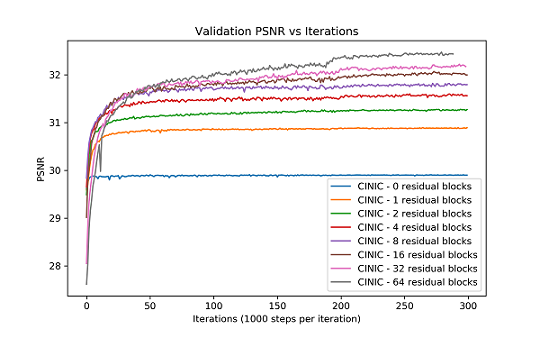
\includegraphics{res-psnr.png}}
  \caption{PSNR values on the validation set over time. Each network has a variable number of residual blocks but 64 filters per convolutional layer}
  \label{fig:res-psnr}
\end{figure}

\begin{figure}[htbp]
  \centerline{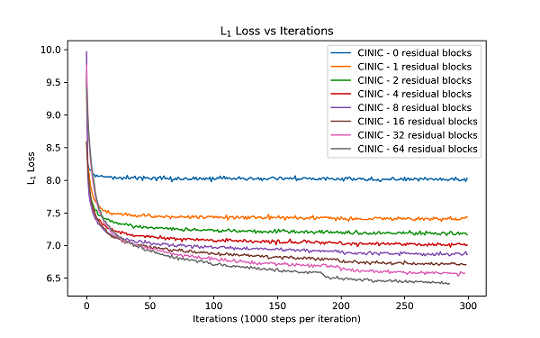
\includegraphics{res-loss.png}}
  \caption{Loss values on the training set over time. Each network has a variable number of residual blocks but 64 filters per convolutional layer}
  \label{fig:res-loss}
\end{figure}

\begin{table}[htbp]
  \centering
  \caption{Each network testing in this table has 64 filters per convolutional layer. These networks were tested on taking 128x128 images and upscaling them to 256x256.}
  \label{tab:res}
  \begin{tabular}{c|c|c|c|c}
    Res. Blocks & sec / epoch & PSNR     & $L_1$ Loss & Parameters \\ \hline
    0           & 6.11        & 29.91 dB & 7.98       & 188,163    \\
    1           & 7.68        & 30.89 dB & 7.37       & 262,019    \\
    2           & 9.48        & 31.28 dB & 7.16       & 335,875    \\
    4           & 12.63       & 31.60 dB & 6.97       & 483,587    \\
    8           & 19.23       & 31.82 dB & 6.84       & 779,011    \\
    16          & 31.93       & 32.07 dB & 6.70       & 1,369,859  \\
    32          & 57.25       & 32.22 dB & 6.53       & 2,551,555  \\
    64          & 105.15      & 32.47 dB & 6.41       & 4,914,947  \\
  \end{tabular}
\end{table}

The third experiment we want to perform is increasing the number of filters and residual blocks to see if we can match the PSNR of the standard network on our much smaller CINIC-10 dataset.
In Figure \ref{fig:filt-psnr} and Figure \ref{fig:filt-loss}, we explore the relationship between increasing both the number of filters and the number of residual layers on the PSNR of the images the networks produce.
Unfortunately, a server issue caused two of the experiments to end short of the 300,000 steps, but we can still draw some conclusions by the trends of their PSNR values over time.
We can see that increasing the number of filters in the network is what really helps increase the PSNR the mode.
The network with 16 residual blocks and 512 filters per convolutional layer was on track to reach the performance of the standard network on DIV2K.
According to Table \ref{tab:filt}, it reached a maximum of 34.51 dB on the validation set before the server error occurred.
And the network with 32 residual blocks and 512 filters was on track to beat both of them.
Unfortunately, the time it takes to train such massive networks is more than most people have without a large number of powerful GPUs or no other training tasks to perform.
It took an average of 881.86 seconds per 1,000 training steps just to train the large network and it have over 160 million parameters which takes up a very large amount of GPU VRAM.

\begin{figure}[htbp]
  \centerline{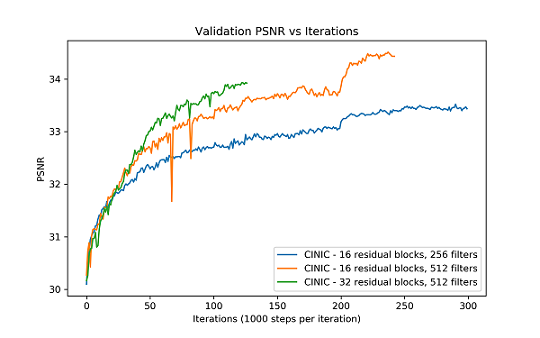
\includegraphics{filt-psnr.png}}
  \caption{PSNR values on the validation set over time. Each network has 16 or 32 residual blocks and 256 or 512 filters per convolutional layer. This is intended to try to find the best possible performance possible on such a small dataset like CINIC-10}
  \label{fig:filt-psnr}
\end{figure}

\begin{figure}[htbp]
  \centerline{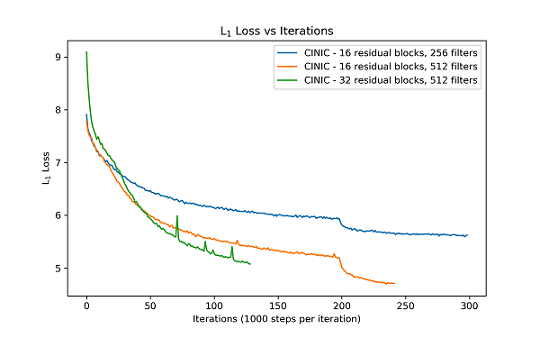
\includegraphics{filt-loss.png}}
  \caption{Loss values on the training set over time. Each network has 16 or 32 residual blocks and 256 or 512 filters per convolutional layer. This is intended to try to find the best possible performance possible on such a small dataset like CINIC-10}
  \label{fig:filt-loss}
\end{figure}

\begin{table}[htbp]
  \centering
  \caption{These networks were tested on taking 128x128 images and upscaling them to 256x256.}
  \label{tab:filt}
  \begin{tabular}{c|c|c|c|c|c}
    Res. Blocks & Filters & sec / epoch & PSNR     & $L_1$ Loss & Parameters  \\ \hline
    16          & 256     & 150.96      & 33.52 dB & 5.59       & 21,847,043  \\
    16          & 512     & 477.09      & 34.51 dB & 4.70       & 87,341,059  \\
    32          & 512     & 881.86      & 33.93 dB & 5.08       & 162,854,915 \\
  \end{tabular}
\end{table}

The last experiment we want to run is related to our main goal of whether or not we can reduce the number of parameters low enough to run on a low compute device like a phone and still out perform bicubic upscaling.
In Figure \ref{fig:min-psnr} and Figure \ref{fig:min-loss}, we explore how small we can make our network in terms of parameters and convolutional filters while trying to keep PSNR above 29.24 dB.
The network with only 1 filter per layer performed abysmally at 22 dB, and the 2 filter network performed worse than bicubic upscaling at 28 dB.
According to Table \ref{tab:min}, a minimum of 4 filters per convolutional layer is needed to reach a PSNR above 29.85 dB, which beats bicubic upscaling!
And it only required 963 parameters to run, which is less than 4KB of memory, low enough to run on a low compute device.

\begin{figure}[htbp]
  \centerline{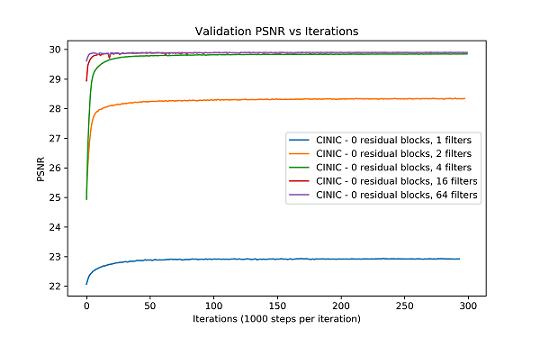
\includegraphics{min-psnr.png}}
  \caption{PSNR values on the validation set over time. Each network has 0 residual blocks and a variable number of filters per convolutional layer. This is intended to try to find the smallest possible network that can outperform bicubic upscaling}
  \label{fig:min-psnr}
\end{figure}

\begin{figure}[htbp]
  \centerline{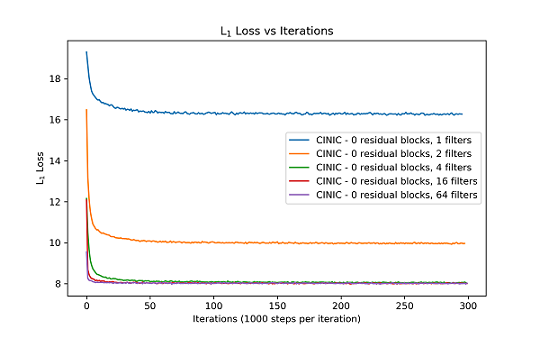
\includegraphics{min-loss.png}}
  \caption{Loss values on the validation set over time. Each network has 0 residual blocks and a variable number of filters per convolutional layer. This is intended to try to find the smallest possible network that can outperform bicubic upscaling}
  \label{fig:min-loss}
\end{figure}

\begin{table}[htbp]
  \centering
  \caption{Each network in this table has 0 residual blocks and a variable number of filters per convolutional layer. These networks were tested on taking 128x128 images and upscaling them to 256x256.}
  \label{tab:min}
  \begin{tabular}{c|c|c|c|c}
    Filters & sec / epoch & PSNR     & $L_1$ Loss & Parameters \\ \hline
    1       & 3.57        & 22.93 dB & 16.22      & 108        \\
    2       & 3.59        & 28.35 dB & 9.93       & 303        \\
    4       & 3.56        & 29.85 dB & 8.02       & 963        \\
    16      & 3.54        & 29.90 dB & 7.98       & 12483      \\
    64      & 6.11        & 29.91 dB & 7.98       & 188163     \\
  \end{tabular}
\end{table}

\section{Conclusion}
In conclusion, we've ran four experiments to determine how well current Single Image Super Resolution networks perform on very small images.
We've shown that the commonly used EDSR is capable of producing high PSNR super resolution images on a very small, 256x256 dataset.
We've also shown that with enough compute power we can push EDSR to its full limits and reach DIV2K-like performance of 35 PSNR if we use 32 residual blocks and 512 filters per convolutional layer.
And, most importantly, we've shown that with a very small network with no residual blocks and just 4 filters per convolutional layer, we can beat bicubic upscaling and deploy that solution to low compute devices since the network has less than 1,000 parameters.

\begin{thebibliography}{00}
  \bibitem{b1} B. Lim, S. Son, H. Kim, S. Nah and K. M. Lee, "Enhanced Deep Residual Networks for Single Image Super-Resolution," 2017 IEEE Conference on Computer Vision and Pattern Recognition Workshops (CVPRW), Honolulu, HI, 2017, pp. 1132-1140.
  \bibitem{b2} E. Agustsson and R. Timofte, "NTIRE 2017 Challenge on Single Image Super-Resolution: Dataset and Study," 2017 IEEE Conference on Computer Vision and Pattern Recognition Workshops (CVPRW), Honolulu, HI, 2017, pp. 1122-1131.
  \bibitem{b3} Darlow L.N., Crowley E.J., Antoniou A., and A.J. Storkey (2018) CINIC-10 is not ImageNet or CIFAR-10. Report EDI-INF-ANC-1802 (arXiv:1810.03505).
  \bibitem{b4} Turkowski, Ken; Gabriel, Steve (1990). "Filters for Common Resampling Tasks". In Glassner, Andrew S. (ed.). Graphics Gems I. Academic Press. pp. 147–165. CiteSeerX 10.1.1.116.7898. ISBN 978-0-12-286165-9.
  \bibitem{b5} Chao Dong, Chen Change Loy, Kaiming He, Xiaoou Tang. Learning a Deep Convolutional Network for Image Super-Resolution, in Proceedings of European Conference on Computer Vision (ECCV), 2014
  \bibitem{b6} W. Shi et al., "Real-Time Single Image and Video Super-Resolution Using an Efficient Sub-Pixel Convolutional Neural Network," 2016 IEEE Conference on Computer Vision and Pattern Recognition (CVPR), Las Vegas, NV, 2016, pp. 1874-1883.
\end{thebibliography}


\section*{Code Design}
I started with a model made by https://github.com/krasserm/super-resolution.
I also used his trainer and dataset as starting points.
Since then the code has been heavily edited to the point of no longer really looking like his.
Emphasizing the specific parts I've written myself or modified heavily for my purposes would almost encompass every line of code be longer than the code itself.
\begin{python}
  # Selects random CINIC images for the experiment.
  # Uses a Python implementation of Matlab's image
  # resize to resize images before saving them.
  # Written completely by me
  prep_cinic.py
  # Loads DIV2K and CINIC images into a tensorflow
  # dataset. Used for training and loading
  # differently scaled images. Originally written
  # by krasserm, but has been heavily modified and
  # added to by me.
  datasets.py
  # Trains an EDSR model given a set of hyper
  # parameters. Saves the best model weights and
  # keeps stats of performance.
  # Written completely by me
  train.py
  # Assists in training and handles the low level
  # backprop as well as keeping checkpoints of the
  # model's weights and stats about training
  # Originally written by krasserm, but has been
  # heavily modified and added to by me.
  trainer.py
  # Contains the actual model architecture of EDSR
  # Written by krasserm, but has been slightly
  # modified and added to by me.
  edsr.py
  # A Python implementation of Matlab's imresize
  # needed to get the EDSR model to work. Why it
  # only works with that imresize is still a
  # mystery.
  # Written by https://github.com/fatheral/
  # matlab_imresize/blob/master/imresize.py
  imresize.py
  # Contains graphs and results needed for Section 6
  Results.ipynb
\end{python}

\section*{Workload Distribution}

I did all the work for this project since I worked alone.

\end{document}
